\chapter{Storyboardy}

Na vytvoření uživatelských skupin a~HTA diagramů navážeme tvořením Storyboardů. Storyboard je náčrt sekvence kroků, které uživatel v~aplikaci provádí. Každý důležitý bod je zaznamenán do buňky. Ty pak skládáme lineárně za sebe, až nám vznikne příběh připomínající komiks. Takové rozdělení umožňuje soustředit se na každý krok zvlášť. Zároveň se jedná o~další techniku, kde můžeme udělat rychlý náčrt a~podle potřeby upravovat. Jeden storyboard nezabere víc než jednu stránku.

Cílem storyboardu je zjednodušeně zobrazit problém co se uživatel snaží v aplikaci řešit a zamyslet se nad jeho přístupem k danému problému. Jde nám hlavně o~vizuální zobrazení konkrétních kroků, které jsme popisovali v~HTA diagramech. Zároveň nám může být návrh nápomocný, abychom si vizualizovali, jak budou uživatelé používat navrhovanou aplikaci a jak bude aplikace v náznacích vypadat. Získané představy a vizualizace použijeme v detailnějším návrhu rozhraní a budeme se k nim snažit přiblížit.

V našem případě vezmeme reprezentanta každé skupiny uživatelů a~představíme si jeho chování pro jednu vybranou situaci z~námi vytvořeného HTA diagramu.

\section{Ukázka vytváření storyboardu}

Jako první začneme se zkušeným uživatelem. V aplikaci bude přidávat dvě různé databázové komponenty (PostgreSQL, MongoDB). Strukturu kroků zachováváme podobnou prvnímu hta (\ref{obr03:hta1}). Chceme zachytit uživatele, který se umí pohybovat v doméně, jenom nepoužíval náš nástroj.

Na Obrázku \ref{obr04:storyboard-1-text} můžeme vidět rychlý návrh obsahu storyboardu. Kroky v buňkách nejdřív místo kreslení popisujeme. Získáme tím přehled všech hlavních kroků, které bude uživatel dělat a ujasníme si, kolik asi bude potřeba buněk.

\begin{figure}[htb]
    \centering
    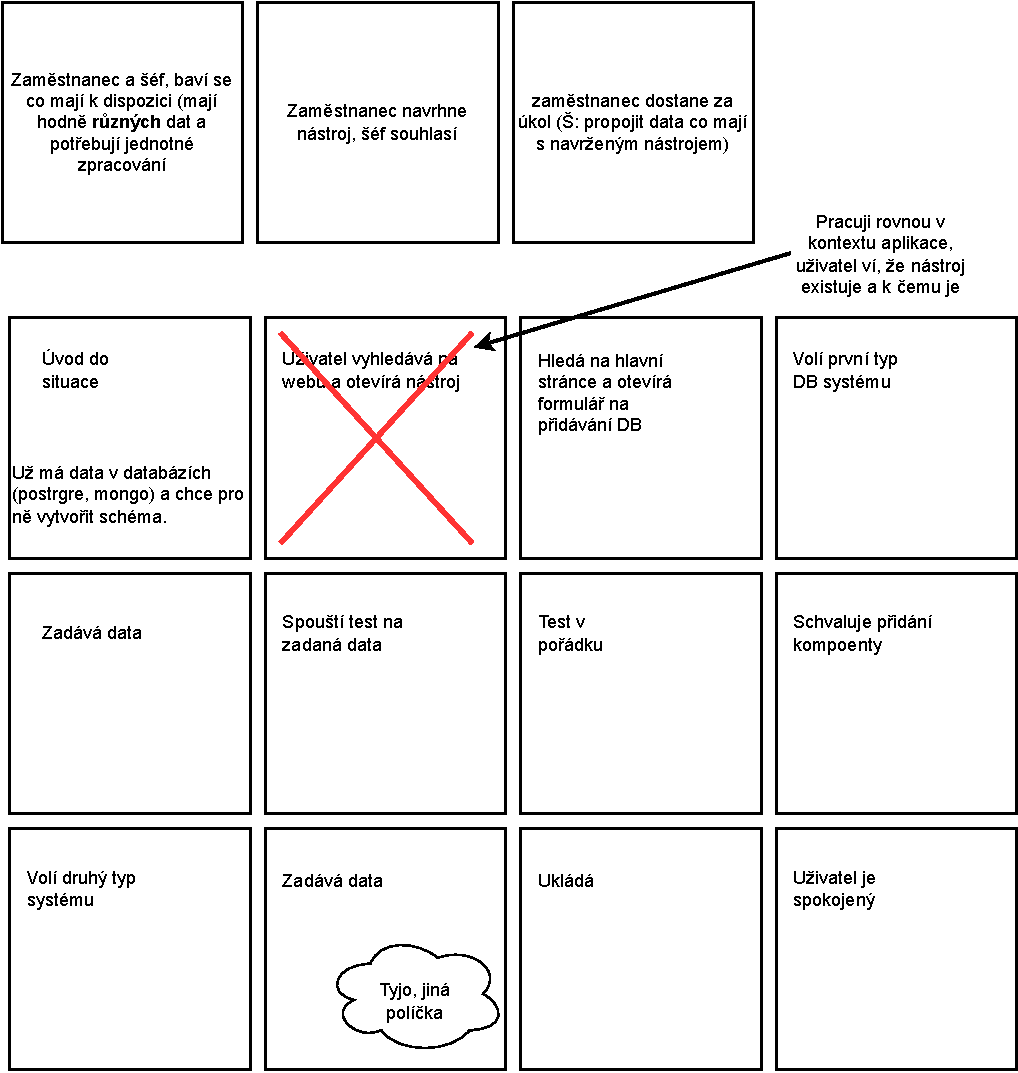
\includegraphics[height=150mm]{../img/storyboard-1-rychly-navrh}
    \caption{Rychlý návrh storyboardu pomocí textu v buňkách.}
    \label{obr04:storyboard-1-text}
\end{figure}

V rámci návrhu jsme vytvořili několik iterací. Některé snímky jsme z návrhu vyřadili, protože nebyli potřebné (např. červeně škrtlý snímek). První tři kroky jsme k původnímu návrhu přidávali jako širší úvod do situace.

Dáváme si pozor, abychom se v této fázi návrhu nenechali strhnout detaily, které zatím nejsou potřeba. O prvotních fázích návrhu se zmiňuje i kniha Refactoring UI \cite{Refactoring_UI}. Navrhuje jednoduchý způsob, jak se nenechat pohltit detaily jako jsou typy písma, stíny, ikony atd. Podle autorů stačí vzít papír, tlustou fixu a tím si v podstatě znemožnit kreslení malých detailů. My jsme navíc omezení velikostí buněk, do kterých kreslíme.

Při vyjadřování situace pamatujeme na to, že aplikaci momentálně ovládá zkušený uživatel. V  aplikaci se zorientuje rychle a s úkolem nemá problém. Obrázek \ref{obr04:storyboard-1} je kompletní storyboard znázorněný pomocí kreseb místo textu. V návrhu je vidět, že uživatel nemá s používáním aplikace problém. Sám navrhl použití nástroje. Na několika snímcích je vidět i prvotní rozhraní aplikace, zatím opravdu jen v náznacích.

\begin{figure}[htb]
    \centering
    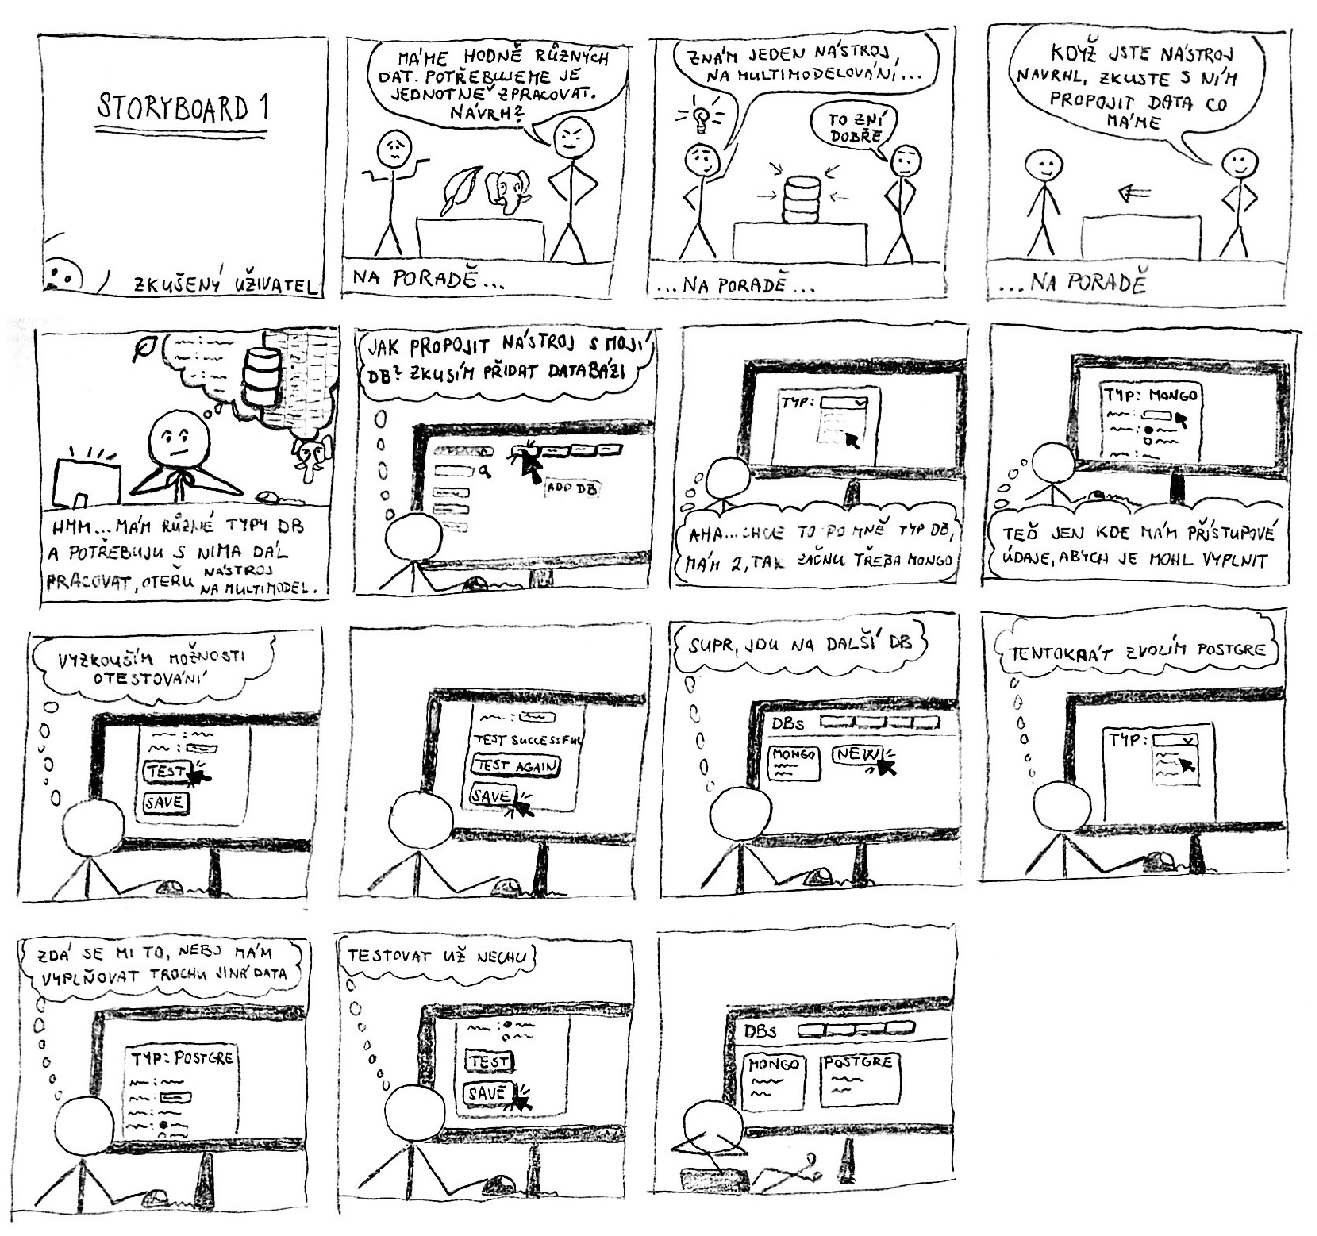
\includegraphics[height=130mm]{../img/storyboard-1}
    \caption{\centering Výsledný storyboard, který znázorňuje uživatele přidávajícího databázové komponenty}
    \label{obr04:storyboard-1}
\end{figure}

Oproti Obrázku \ref{obr04:storyboard-1-text} si díky vizualizaci v Obrázku \ref{obr04:storyboard-1} lépe představíme co bude uživatel dělat a jak bude v náznacích vypadat aplikace, ve které pracuje. Stejně tak se potom konkrétní představy lépe komunikují s lidmi se kterými storyboard konzultujeme.
